\section*{Reglas de Negocio para el Sistema de Gestión de Trabajos Terminales}

\begin{tabular}{ | m{3cm} | m{12cm} | } 
\hline
\textbf{Identificador} & \textbf{Reglas de Negocio} \\
\hline
RN01 & Cada equipo de alumnos puede tener hasta 3 integrantes. \\
\hline
RN02 & Cada trabajo terminal puede tener hasta 4 profesores sinodales asignados. \\
\hline
RN03 & Un profesor sinodal será elegido aleatoriamente para calificar el trabajo terminal. \\
\hline
RN04 & La propuesta de trabajo terminal debe ser subida a la plataforma por un alumno del equipo. \\
\hline
RN05 & Los profesores deben decidir aceptar o rechazar una propuesta de trabajo terminal aportando retroalimentación. \\
\hline
RN06 & En caso de aceptación de la propuesta, se vincula automáticamente a los alumnos con los profesores. \\
\hline
RN07 & Los profesores y alumnos pueden agendar y modificar citas a través de la plataforma. \\
\hline
RN08 & La calificación y comentarios del profesor sinodal deben darse en un máximo de tres días después de la evaluación. \\
\hline
RN09 & Solo se permite la subida de documentos en formatos específicos (PDF, DOCX, etc.). \\
\hline
RN10 & Los alumnos deben estar inscritos en la institución para poder utilizar el sistema. \\
\hline
RN11 & Los profesores deben estar activos en la institución para participar en el sistema. \\
\hline
RN12 & Los trabajos terminales rechazados dos veces serán dados de baja automáticamente del sistema. \\
\hline
RN13 & La plataforma debe estar disponible para acceso excepto en días festivos y vacaciones. \\
\hline
RN14 & Los datos personales de alumnos y profesores deben ser protegidos según las normativas de privacidad aplicables. \\
\hline
RN15 & La integración con la plataforma SAES debe ser mantenida para la verificación y recopilación de datos. \\
\hline
\end{tabular}

\newpage

\section*{Reglas de Negocio para el Sistema de Gestión de Trabajos Terminales}
\begin{figure}[!h]
    \centering
    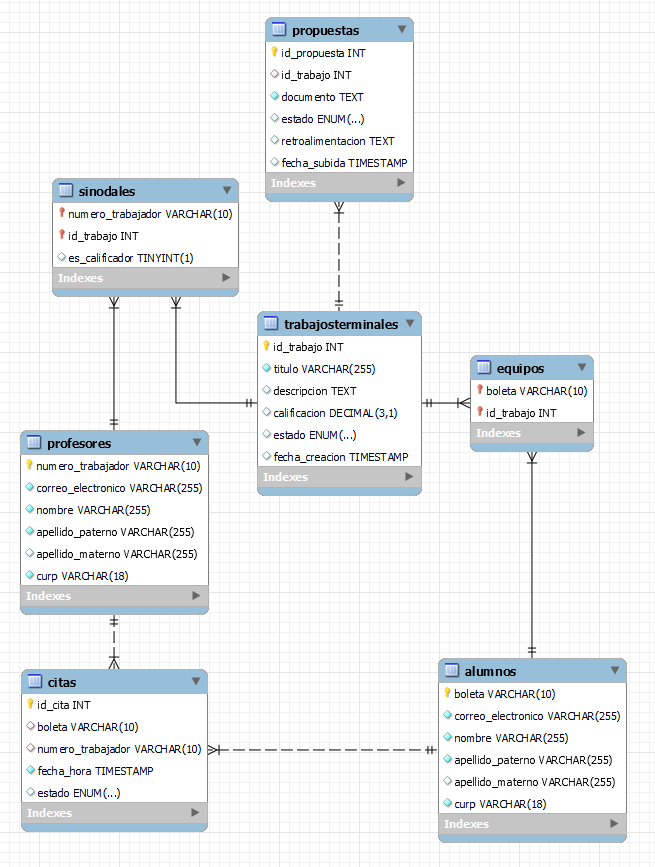
\includegraphics[scale = .87]{bd.png}
\end{figure}